\RequirePackage{fix-cm}
\documentclass[conf]{new-aiaa}

\usepackage[utf8]{inputenc}
\usepackage{hyperref}
\usepackage{graphicx}
\usepackage{siunitx}
\sisetup{group-separator = {,}}
\usepackage{booktabs}
\usepackage{enumitem}
\usepackage{float}
\usepackage{amsmath}
\usepackage[version=4]{mhchem}
\usepackage{longtable,tabularx}
\usepackage{placeins}
\usepackage{multirow}
\usepackage{booktabs}
\usepackage{latexsym}
\usepackage{subcaption}
\usepackage{latexsym}
\usepackage[sort&compress,numbers]{natbib} % For bibtex \citet, \citep
\usepackage{hypernat} % To get natbib to play nicely with hyperref
\usepackage{doi} % For getting hyperlinked DOI in the references


\hypersetup{
    pdfauthor={Peter Atma}, % insert author here
	pdftitle={Aviation 2022 Abstract}, % insert title here
	pdfsubject={Propulsion Analysis and Optimization of an Ultra Bypass Turbofan Engine}, % insert keywords here
}

\graphicspath{{../figures/}}

\title{Comparing Hydrogen and Jet-A for a Ultra High-Bypass Turbofan with Water Recirculation} % change

\author{Peter Atma\footnote{MSE Student, Department of Aerospace Engineering, AIAA Student Member}}
\author{Andrew H.R. Lamkin\footnote{Ph.D.~Candidate, Department of Aerospace Engineering, AIAA Student Member}}
\author{Joaquim R.~R.~A.~Martins\footnote{Professor, Department of Aerospace Engineering, AIAA Fellow}}
\affil{University of Michigan, Ann Arbor, MI, 48109}

% ==================================================
%	Abstract
% ==================================================

% ==================================================
\begin{document}

\maketitle

\begin{abstract}
	Advances in commercial propulsion technology have resulted in the creation of larger and more advanced high-bypass turbofan engines with higher bypass ratios, pressure ratios, and internal temperatures.
	With the focus on reducing aircraft emissions, aircraft and engine manufacturers have been pushing for Hydrogen as a fuel and more efficient engines to lower carbon dioxide and NOx emissions.
	Using Hydrogen introduces complexity and weight penalties that we need to offset by using all the advantageous properties of the fuel.
	In this study we investigate the benefits of using Hydrogen versus Jet-A fuel with a closed-loop water recirculation system within a high-bypass turbofan.
	We will setup and perform a gradient-based optimization parameter sweep to understand the performance and emissions benefits of water recirculation using Jet-A and Hydrogen fuels.
	This study will demonstrate the benefits of hydrogen combustion with water recirculation in order to encourage next-generation propulsion systems to use the properties of hydrogen for improved performance and reduced emissions.
\end{abstract}

\section{Introduction}
% Message 1: Motivation to incorporate low-emission fuels and techniques
The effects of climate change are pushing the aviation industry towards Hydrogen-fueled propulsion systems as a solution to reduce emissions.
N+3 technology estimates for turbofan engines that burn hydrocarbon fuels suggest that higher efficiency can be achieved by designing ultra high-bypass (UHB) engines with small cores and high overall pressure ratios (OPR).
Higher OPR and smaller core designs are pushing the limits of compressor and turbine design, placing an upper bound on potential performance and emissions improvements.
Switching to hydrogen as the primary fuel source reduces carbon dioxide emissions immediately, but adds complexity and weight that offset the benefits.
However, Hydrogen is a versatile fuel with advantageous chemical and thermodynamic properties that can be leveraged to further increase the performance and emission reduction of the propulsion system.
In this study, we investigate the tradeoff between burning hydrocarbon fuels like Jet-A or Hydrogen considering UHB ratio turbofan engines.
We will look at new ideas with water recirculation to further squeeze performance and efficiency from Jet-A and Hydrogen combustion using gradient-based design optimization.
% TODO: AL-PA: We don't need this sentence until later.
% Furthermore, higher overall pressure ratios and more advanced metals with higher melting temperatures can allow larger burner temperatures both of which improve thermal efficiency.

% Message 2: Background and references to support using H2 and water injection in HBTF engines
Water recirculation is the process of extracting water from the exhaust stream of a propulsion system and injecting it upstream of the combustor as finely atomized droplets.
NASA, Boeing, and Rolls-Royce studied this concept and suggested that this technique reduces the NOx emissions as much as 47 percent.
Additionally, water recirculation improves fuel efficiency and thrust output with lower burner temperatures that can improve the lifetime of turbine blades and reduce noise~\cite{nasa_inject}.
Traditional propulsion systems that burn hydrocarbon fuels would require external water storage on the aircraft because they do not produce enough in the exhaust for recirculation.
The added weight of tanks, pumping, and ducting makes this concept infeasible for a conventional aircraft.
However, if Hydrogen fuels are used, the main product of Hydrogen combustion is water vapor and can thus be recovered.
The ability to recirculate water vapor from the exhaust of hydrogen combustion reduces the requirement for storage tanks and allows for the creation of a closed loop system inside the propulsion cycle.

Zero-dimensional cycle modeling is an efficient tool for predicting the initial design, performance, and emissions of new propulsion concepts.
Zero-dimensional cycle analysis uses a first-principles approach with a chemical equilibrium analysis (CEA) thermodynamics solver that considers the molecular species of different fuels.
This can be used to understand the trends and design limitations of an engine cycle and study potential improvements in design using optimization.
The industry standard for zero and one-dimensional cycle analysis is the Numerical Proprulsion System Simulation (NPSS) framework~\cite{JonesNPSS}.
NPSS is a modular object-oriented framework in that models engine components as individual blocks with several thermodynamic solvers.
\citet{Hendricks2019} and \citet{Gray2017b} created a tool called pyCycle with the same functionality as NPSS, but including analytical derivatives for every engine component and thermodynamic solver.
We use pyCycle because it is built on top of the OpenMDAO framework~\cite{Gray2019a} to simplify gradient-based optimization and leverage hierarchical nonlinear solver structures to improve robustness.

% Message 3: Introduce the extension of the HBTF and propose novel contributions
In this work, we will analyze the potential propulsion benefits of a closed-loop water vapor recirculation with a water injection system in a high-bypass turbofan engine by optimizing the thrust-specific energy consumption (TSEC) with a NOx emission constraint.
TSEC is the thrust specific fuel consumption multiplied by the lower heating value of the fuel and is a metric for comparing the efficiency of different fuel choices.
We will develop new pyCycle components for water injection and vapor recovery within pyCycle to understand the benefit of a closed loop recirculation system.
In addition, we will apply existing empirical models as well as develop new surrogate models to estimate NOx emissions using chemical reactor networks and steady-state combustion analyses.
Finally, we will present a comparison between Jet-A and hydrogen combustion with and without water recirculation in terms of improvement of TSEC and emissions.

In Section \ref{sec:epModel} we introduce the turbofan model and explain how we will implement the water injection and water recovery components in pyCycle.
Section \ref{sec:imp} explains the implementation of the multi-point optimization problem and the conditions limiting the engine model.

\section{Emission-Propulsion Model Description}
\label{sec:epModel}
% Engine Architecture: Describe the flow path of the engine and establish the mechanical coupling.
We will use a next-generation UHB turbofan engine configuration for this work.
Specifically, the NASA advanced technology high bypass geared turbofan engine cycle, referred to as the "N+3" engine, was selected for this research \cite{Jones2017a}.
The N+3 reference cycle represents a UHB ratio geared turbofan that could be available in the 2030–2040 time frame.
This engine was selected since it has already been modeled in pyCycle as a robust example cycle and includes the advanced engine cycle improvements such as a large bypass ratio, high pressure ratio, and high combustion temperature.
The flow path consists of an inlet that directs ambient air through a fan, followed by a duct that splits the flow into a core flow and a bypass flow, each of which ends in a bypass nozzle and core nozzle, respectively.
The fan and low pressure compressor (LPC) are connected to the low pressure turbine (LPT) by the low pressure shaft and the high pressure compressor (HPC) is connected to the high pressure turbine (HPT) by the high pressure shaft.
Along the axial flow path, the zero-dimensional thermodynamic connections are solved using CEA to ensure first the principle governing equations are satisfied.
The closed-loop water recovery system is implemented into the cycle by placing a water injection component directly before the HPC.
This component will inject pure water into the core stream which will reduce the combustion temperature due to heat absorption from vaporization.
The water vapor recovery component is placed directly before the core nozzle to extract water from the core stream and recycle it back to the water injector.
In practice a water vapor recovery component requires a complex condenser model in the core stream, this work will only look at the potential benefits of extracting water vapor and not the recovery method specifically.
The component flow interface and mechanical connections, including the water injector and water extractor, are depicted in Figure \ref{fig:hbtf_cycle}.

% TODO: AL-PA: You need to add more description to the caption.  The figure and caption should stand alone in the paper.
% i.e The reader should be able to look at the figure and caption and understand without reading the paper.
% It's okay for the caption to be 3-4 sentences long if necessary.
\begin{figure}[H]
	\centering
	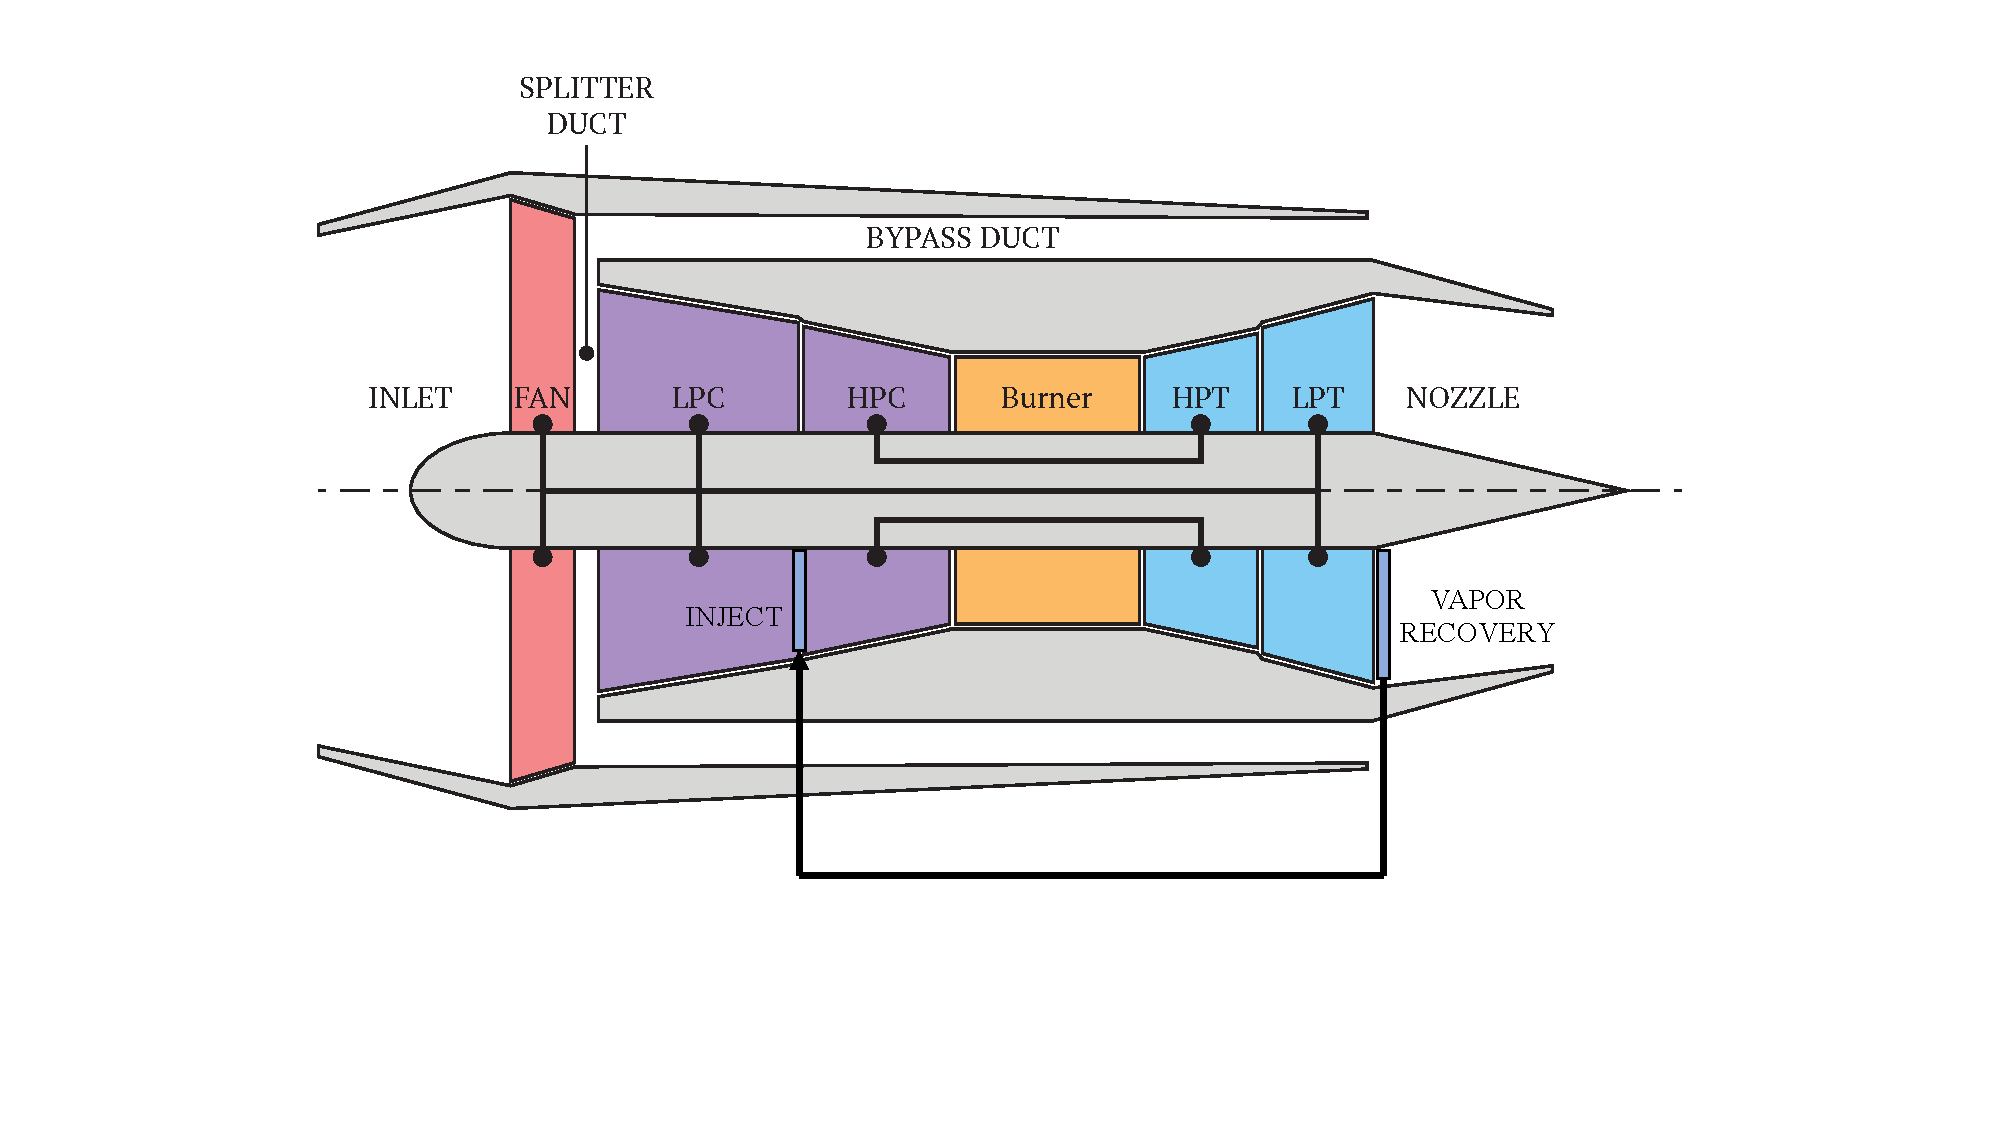
\includegraphics[width=0.8\textwidth]{turbofan_wvr.pdf}
	\caption{The configuration of a high-bypass turbofan model with an integrated closed-loop vapor recovery and injection system.
		Water vapor is recovered from the core stream of the engine before the nozzle and is re-injected into the core stream before the LPC.}
	\label{fig:hbtf_cycle}
\end{figure}

% Preliminary Results
We tested the N+3 propulsion model with water injection using Jet-A and liquid hydrogen fuels to determine if there are any immediate improvements in efficiency.
The preliminary results from this analysis are shown in Figure \ref{fig:results} and show the relative improvement in TSEC with water injection for the same engine design with each type of fuel.
We see improvements in the cruise engine efficiency using a baseline analysis and will be further improved using design optimization.

% TODO: AL-PA: Again, this needs a much better caption.
\begin{figure}[H]
	\centering
	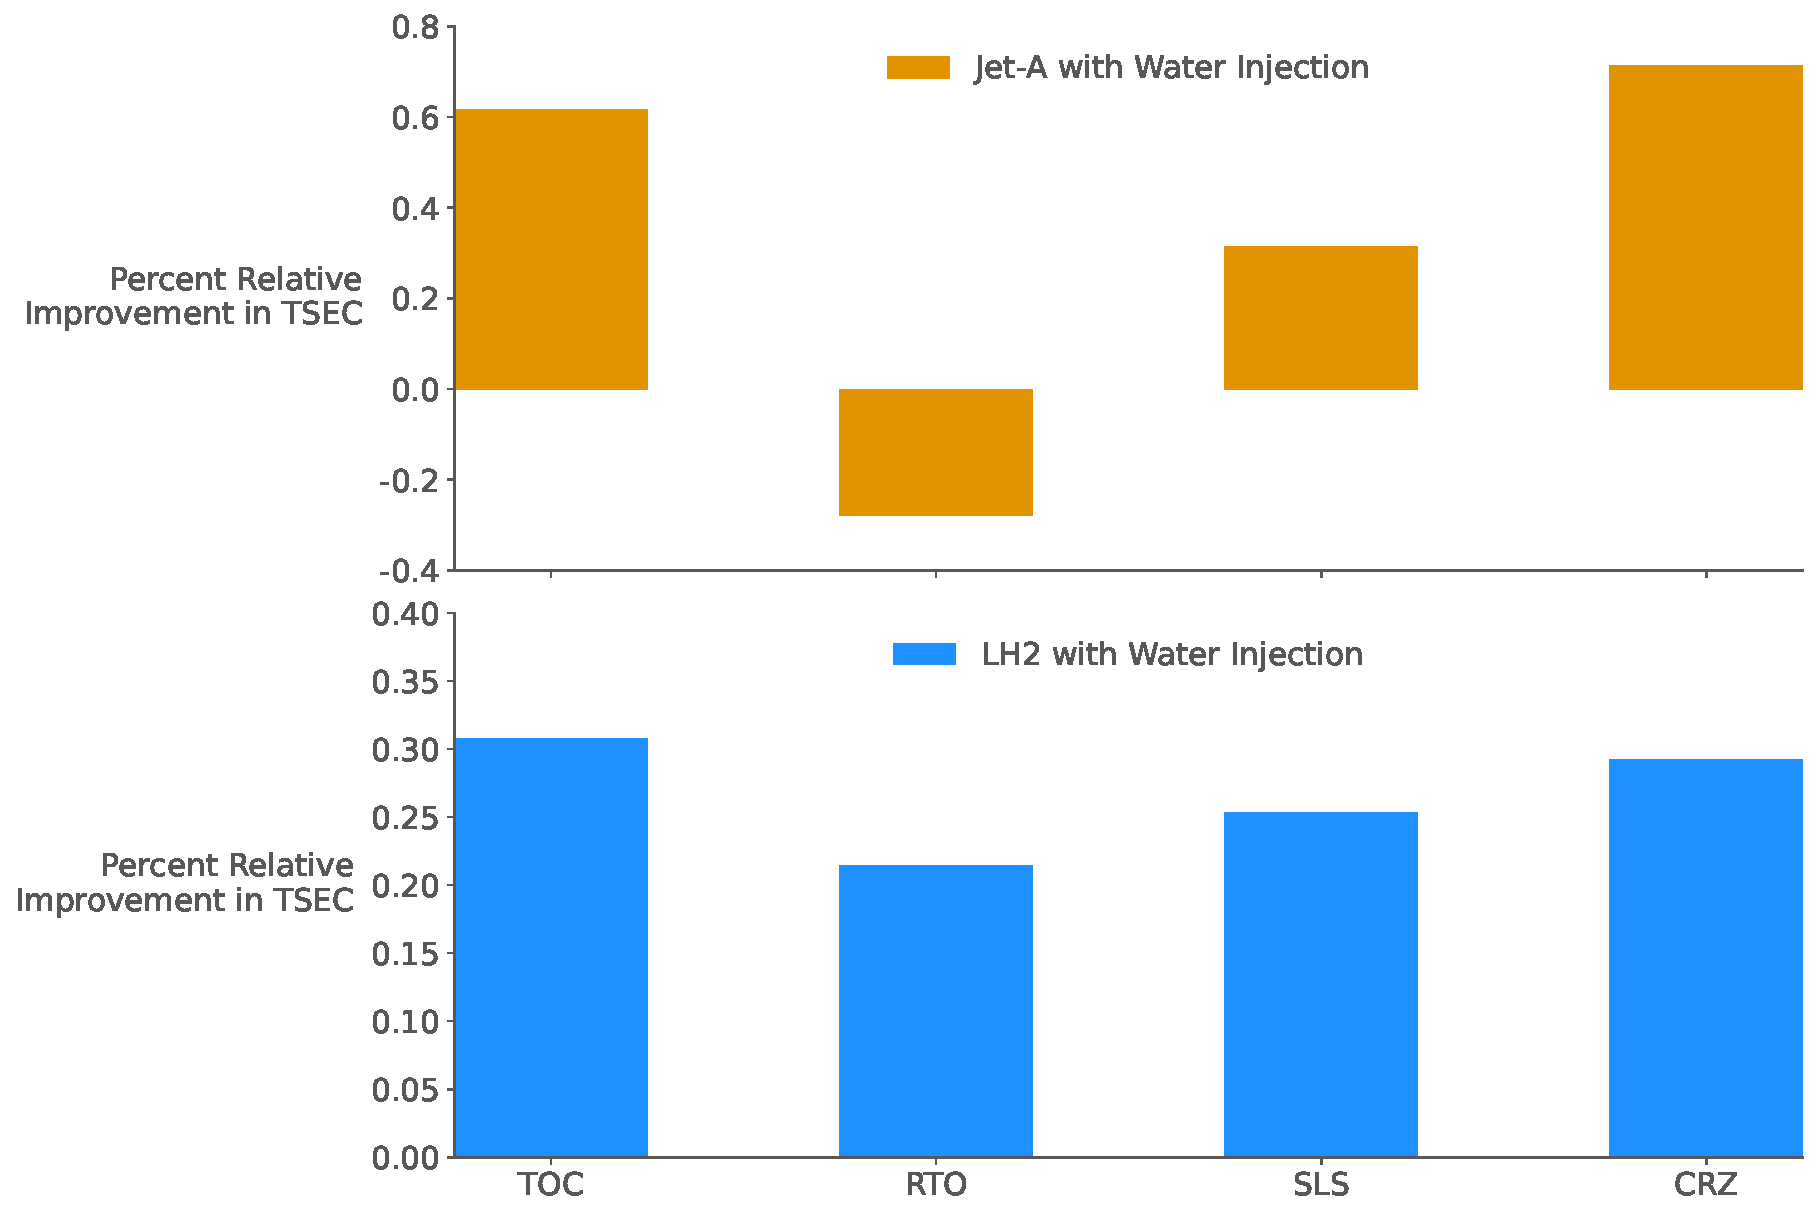
\includegraphics[width=0.8\textwidth]{JetA-H2_bar_chart_diff.pdf}
	\caption{Percent relative improvement in thrust specific energy consumption (TSEC) of an ultra-high bypass turbofan engine from water injection.
		Data was collected with and without water injected into the core stream of the engine for Jet-A and hydrogen fuels.}
	\label{fig:results}
\end{figure}

\section{Implementation}
\label{sec:imp}
% Fully coupled model
The propulsion model is constructed in pyCycle which is built on top of OpenMDAO to allow a modular design of the engine components and allows the coupling of other engineering disciplines for analysis \cite{Gray2019a}.
The NOx model for Jet-A fuel will use the P3-T3 method~\cite{Dubois2006}, a common technique in academia and industry for determing NOx formation in aircraft engines.
This method uses the pressure and temperature of the flow before the combustor to determine NOx formation.
Since not many accurate NOx formation correlations exist for full-sized turbofan engines running on liquid hydrogen, we will use a surrogate model using data from combustor reactor network models to accurately predict NOx emissions.

% Briefly discuss the optimization problem
We will perform gradient-based emission-propulsion design optimization of the engine model with a multi-point architecture that considers several flight conditions experienced by commercial aircraft.
An XDSM diagram of the optimization problem with the multi-point formulation is shown in Figure \ref{fig:opt_prob}.

\begin{figure}[H]
	\centering
	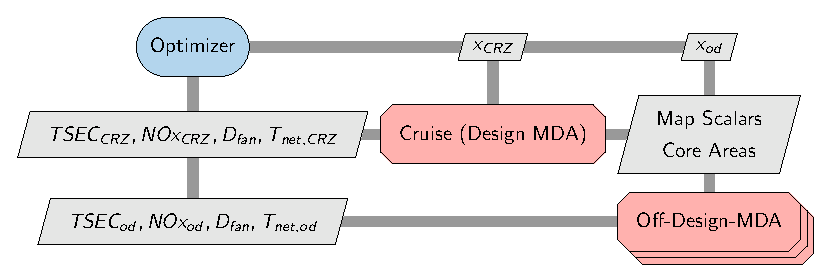
\includegraphics[width=0.8\textwidth]{N3_inject.pdf}
	\caption{XDSM diagram of the multi-point optimization problem with constraints.
		The XDSM diagram shows the variables and outputs within the optimization model and how each of these values is connected to the optimizer and design points.}
	\label{fig:opt_prob}
\end{figure}

The objective is to minimize the TSEC at a cruise condition subject to constraints on NOx formation, thrust, max temperature, and engine diameter.
We will perform a parameter sweep of the limiting constraint to understand the impact of different emissions and performance requirements on the design space.
With an understanding of the design space, we will construct a multi-objective optimization problem to generate a pareto-front for the trade-space between TESC and NOx emissions.

\section{Conclusion}
% Message 1: Re-state the problem
In this work, we will model, analyze, and optimize a UHB next-generation turbofan model considering Jet-A and hydrogen fuel using a novel closed-loop water vapor recovery to improve cycle efficiency and NOx emissions.
% Message 2: Summarize the HBTF model
The high-bypass turbofan engine will be composed of separate sub-components modeled in pyCycle with the new water recovery and injection capability to assess the performance and emissions improvements.
We will compare Jet-A and liquid hydrogen with and without the closed-loop water vapor recovery system to determine the benefits of this technology implementation.
The results will show a quantitative comparison at the propulsion system level, with a qualitative assessment of the feasibility of water recirculation for both Jet-A and hydrogen fuels.
We will use existing P3-T3 methods in addition to new surrogate based NOx prediction models to predict the emissions impact of each fuel with and without water recirculation.
% Message 3: Expected results
We will develop a multi-objective optimization problem to find a pareto-front between TESC and NOx emissions for all fuel and water recovery architectures proposed in this work.
Finally, this work will demonstrate the ability of gradient-based optimization with zero-dimensional cycle analysis to explore the potential benefits of hydrogen combustion with a closed-loop water vapor recover and injection.

\bibliography{mdolab,references}

\end{document}